\section{Problems, Challenges and Requirements}

\subsection{What are the usage data?}

System logs contain a wealth of information to help manage systems. Most systems print out  logs during their executions to record system runtime actions and states that can directly reflect system runtime behaviours. System developers and architects usually use these logs to track a system to detect and diagnose system anomalies. However, there are challenges in analyzing system logs in order to understand a system’s behaviors. 
% The program logic of a system usually has a lot of branches, and thus the system’s behaviors may be quite different under different input data or environmental conditions. Knowing the execution behavior under different inputs or configurations can greatly help system operators to understand system behaviors. However, there may be a large number of different combinations of inputs or parameters under different system behaviors. Such complexity poses difficulties for analyzing contextual information related to the state of interest. 
The user-level usage data in the context of this paper is the usage data generated as a result of user interaction with a cloud-based application. Some examples of usage data are  application logs, server logs, VM logs, Web cookies (from web browser), and so on. Such data in the cloud is spread across various interfaces such as Web browser, mobile apps and command line interfaces on the front-end and server and database on the back-end.  
% Generally, each log message consists of two different types of content: a constant string and parameter values. For example, for the first log-printing statement in Table 1, the constant string is “JVM with ID: given task:”, and the printed parameters are JvmId and TaskId. The log messages printed by the same log-print statement contain the same constant string, and are considered to be of the same type, represented by the constant string. 

As summary, there are mainly three sources of usage data can be extracted from the back-end of the cloud system: the system logs from the cloud services, the application logs, and the logs from the VMs. Fig.~\ref{fig:schema} shows a summary of the three main sources of usage data and the answers for the above questions.


\begin{figure*}[t!]
	\centering
	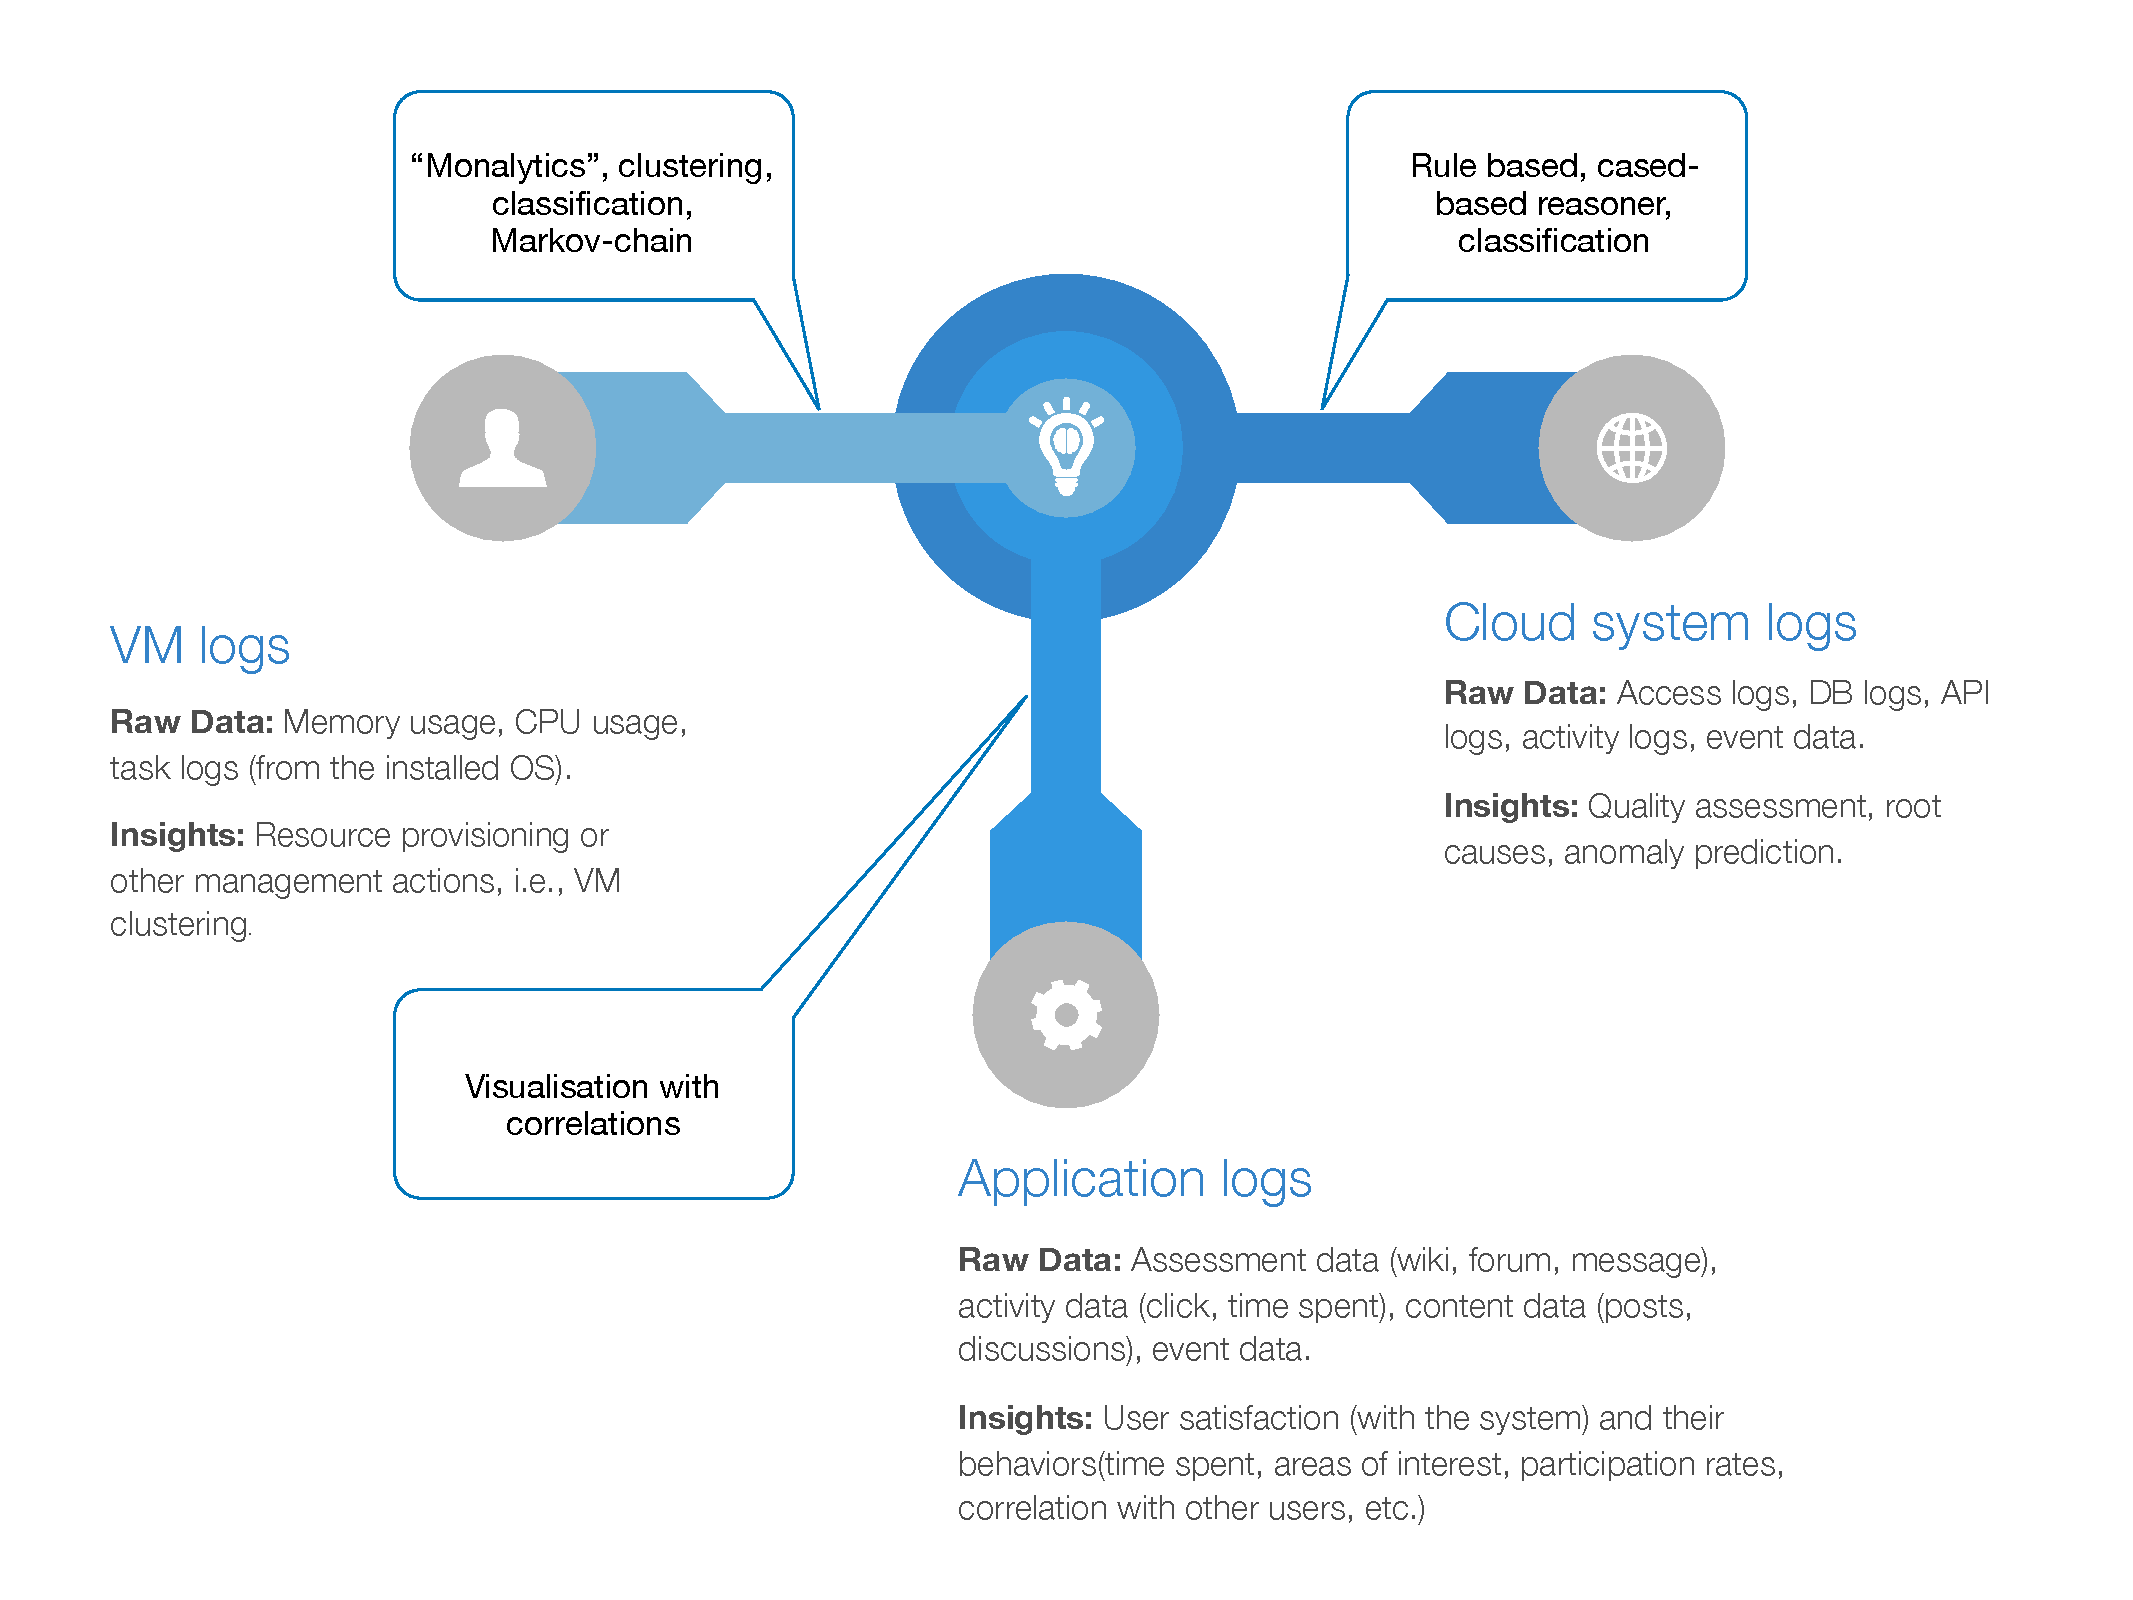
\includegraphics[width=\linewidth]{summary}
	\caption{Three main sources of usage data in cloud-based environment.}
	\label{fig:schema}
\end{figure*}

\subsection{Challenges in Extracting Information from Usage Data}

There are challenges in analyzing system logs in order to understand an end-user’s behaviors. The program logic of a system usually has a lot of branches, and thus the system’s behaviors may be quite different under different input data or environmental conditions. Knowing the execution behavior under different inputs or configurations can greatly help system operators to understand system behaviors. However, there may be a large number of different combinations of inputs or parameters under different system behaviors. Such complexity poses difficulties for analyzing contextual information related to the state of interest. Considering the multi-tenant architecture of the cloud, different applications share the same physical and virtual resources. This raises another challenge as in how to separate and extract the logs that represent each application from the instance (VM) co-hosting the applications. 
%
Since one of the ways to access the cloud-based applications by the end-user is through a web-browser, web-mining techniques can be employed to obtain interaction insights. \cite{Bucklin2009} provide an overview of \emph{Clickstream} data which is defined as the electronic record of a user's activity on the internet, this represents the data trace the path an end-user takes while accessing the cloud application. 

The study in~\cite{Fu2013} proposes a new approach for the contextual analysis of program logs to better understand a system’s behaviors. In particular, they used execution patterns to represent the execution structures reflected by program logs, and propose an algorithm to mine execution patterns from the program logs. The mined execution patterns correspond to different execution paths of the system. Based on the execution patterns, their approach further learns the essential contextual factors (e.g., occurrences of specific program logs with specific parameter values) that cause a specific branch or path to be executed by the system. 
% * <manojpratnas@gmail.com> 2017-11-16T12:04:53.536Z:
% 
% Have to find the reference?
% 
% ^.
%
The mining and learning results can help system operators understand the execution logic and behaviors of a software system for their various maintenance tasks such as system problem diagnosis. This paper makes the following research contributions: We conduct Formal Concept Analysis (FCA) [4] to analyze log messages, and construct a concept lattice graph. The learned graph is used to mine execution patterns and to model relationships among different execution patterns. Such relationships represent branch structures in the program execution logic.

A huge wealth of various data exists in the software development process, and hidden in the data is information about the quality of software and services as well as the dynamics of software development. With various analytic technologies (e.g., data mining, machine learning, and information visualization), software analytics is to enable software practitioners to perform data exploration and analysis in order to obtain insightful and actionable information for data-driven tasks around applications and services.

\subsection{Challenges in Building Usage Analytics Framework}

Despite the advantages provided by analytical solutions, the solution implementation is usually very costly, which hinders enterprises, especially the SMBs (Small and Medium Business), to start such projects. Typically, an enterprise is required to first build a large storage system to store huge volumes of data collected from various data sources and channels; after that, the enterprise should buy expensive analytics software, and a large number of server machines, because the analytical programs often need mining huge amounts of data or executing complex learning algorithms. Moreover, the computational resource demand pattern of analytical solutions may be uneven with spikes (e.g., predicting product sale when a financial quarter is over or some unusual events happen), which means the enterprise has to pay a lot to maintain the complex software and hardware only for occasional usages. As a result, the systematical adoption of analytical solution is currently limited to only a small number of large enterprises. On the other hand, the analytical solution vendors also find it is difficult to deliver cost-effective solutions. Because analytical solutions require continuous model validation, tuning, and update according to the changing business context, it is hard for the solution vendors to control the travel expenditure in sending analysts to conduct incremental services in the customer site. In a word, a cost-effective delivery model becomes an important issue to accelerate the prevalence of analytical solutions. 

Currently, SaaS delivery model is well-studied to enable business clients consume applications at a low cost based on their usage [1], and cloud computing is considered as a promising technology to provide on demand storage and computational resources flexibly [2]. Accordingly, there are several relevant research efforts which have focused on leveraging these technologies to facilitate analytical solution delivery [3][4]. However, most of the projects are ad-hoc, that is, each of them is specific to a certain analytical application domain, and there is still lack of a comprehensive study to identify the differences between existing analytical solution delivery and analytics-as-a-service delivery, as well as a technical framework to handle the technical challenges introduced by the new delivery model.

\subsection{Analytics Requirements}

In~\cite{Paper2013}, the authors pointed general requirements for an usage analytics are detailed below:
\begin{enumerate}
\item Data Source: AE must be able to fetch monitoring data recorded in the database. Further, it must be able to query the Cloud middlewares (e.g., that of OpenStack and OpenShift) and application APIs to know the current status of the services. 	
\item Proactive: AE must support the proactive management of resources. Proactive management needs short term and medium term predictions for the evolution of most relevant metrics. 
\item Alerts: Certain QoS metrics need to be processed in real time and alerts should be triggered when these QoS metrics are violated or approach certain threshold values. 
\item Event Correlation: Detecting the root cause of QoS faults and taking effective counter measures requires monitoring information spanning multiple tiers of the virtualized platforms. Quick in-comprehensive analysis of monitoring data of individual tiers does not reveal the root cause(s) of the problem precisely enough. Therefore, Analytics need to exhaustively aggregate runtime data from different sources and consolidate information at a high level of abstraction. 
\item Identification of Influential Metrics: Identification of the metrics which strongly influence the QoS helps in decreasing the monitoring footprint and analysis complexity.
\item Scalability: The MF should be scalable i.e. it can cope with a large number of monitoring data collectors. This requirement is very important in Cloud Computing scenarios due to a large number of parameters to be monitored for potentially large amount of services and elements of Cloud tiers that may grow elastically. 
\item Heterogeneous data: The MF should consider a heterogeneous group of metrics. The MF must al- low the collection of service level runtime monitoring data, virtual IT-infrastructure monitoring data (e.g., VM level runtime monitoring), and fine-grained physical IT-infrastructure monitoring data (e.g., network links, computing and storage resources). 
\item Relationship: In the above mentioned scenario, clusters of VMs and Physical Machines (PM) serve many kinds of applications, so there is a hierarchical relationship between applications, VMs and PMs.
There is also a possibility of migration of VMs and applications from one node to another, so relation- ships can be changed dynamically. Themetric’s value must be tagged to show that they belong to a particular instance (e.g., application), and what is their relation to other instances (e.g., VM and PM). 
\item Data Repository: The MF requires a data repository where raw monitoring data needs to be stored after collection. The original data set must be stored without down-sampling for auditing purposes. The stored, raw monitoring data can be retrieved by consumers to perform QoS fault diagnosis, SLA validation, plot rendering, and as an input for fine grained resource management. The database must be distributed in order to avoid single point of failure. Moreover, it must be scalable, and allow to store thousands of metrics and potentially billions of data points. 
\item Non-Intrusive: The MF must be able to retrieve data non-intrusively from a variety of sources (for VM via libvirt API, for a host via cgroups, for the network via SNMP, for Java applications via JMX, etc.). Collection mechanism should easily be extensible by adding more plugins. 
\item Interface: The MF should provide a REST interface that allows access to the current monitoring data in a uniform and easy way, by abstracting the complexity of underlying monitoring systems. A standard unified interface for common management and monitoring tasks can make different virtualization technologies and Cloud providers interoperable. A REST interface is a good choice due to ease of implementation, low overhead and good scalability due to its session-less architecture.
\end{enumerate} 

\subsection{Evaluations and Validations}
Evaluation itself is a challenge in usage analytics. For example, if an analytical solution provides some information about the user satisfaction, it is nontrivial to evaluate if that information really show the real ``picture" of the satisfaction from the users. Traditionally, we need to run some surveys to evaluate results from the analytical solutions. Beside of that, in this study, we also propose a novel way for the evaluation by using another usage information, gathering from the snapshots of the users' device, for example screen-shots of the computer. By collecting these information (in the testing phase), we can provide users with the ability to recall and re-access their previous computer usage and the content they engage with. 